\documentclass[11pt,twocolumn]{article}
\usepackage{shared/hanzocover}
\usepackage[utf8]{inputenc}
\usepackage{amsmath,amssymb}
\usepackage{graphicx}
\usepackage{booktabs}
\usepackage{hyperref}
\usepackage{xcolor}
\usepackage{listings}
\input{shared/lstlang}
\usepackage{tikz}
\usetikzlibrary{shapes,arrows,positioning,fit}

\definecolor{codegreen}{rgb}{0,0.6,0}
\definecolor{codegray}{rgb}{0.5,0.5,0.5}
\definecolor{codepurple}{rgb}{0.58,0,0.82}
\definecolor{backcolour}{rgb}{0.95,0.95,0.92}

\lstdefinestyle{mystyle}{
    backgroundcolor=\color{backcolour},
    commentstyle=\color{codegreen},
    keywordstyle=\color{codepurple},
    numberstyle=\tiny\color{codegray},
    stringstyle=\color{codegreen},
    basicstyle=\ttfamily\footnotesize,
    breakatwhitespace=false,
    breaklines=true,
    captionpos=b,
    keepspaces=true,
    numbers=left,
    numbersep=5pt,
    showspaces=false,
    showstringspaces=false,
    showtabs=false,
    tabsize=2
}
\lstset{style=mystyle}

\title{Hanzo Edge: On-Device AI Inference for Mobile and IoT Deployments}
\author{Antje Worring, Hanzo AI Research\thanks{research@hanzo.ai} \\ \textit{Hanzo Industries} \\ \texttt{research@hanzo.ai}}
\date{July 2024}

\begin{document}

\hanzocoverpage

\begin{abstract}
We present Hanzo Edge, a Rust-based inference runtime for deploying AI models on mobile devices, edge servers, and IoT hardware. Edge supports ONNX model loading with automatic optimization for target hardware, including Apple Neural Engine (ANE) on iOS/macOS, GPU compute via Metal and Vulkan, and SIMD-accelerated CPU inference. The runtime implements dynamic quantization (INT8/INT4), operator fusion, and memory-mapped model loading to minimize memory footprint and startup latency. This paper describes those mechanisms and reports no measurements; Section~\ref{sec:figures} records the on-device latency figures an earlier version reported and why they are withdrawn. We describe the hardware abstraction layer, the quantization pipeline, and the model optimization passes that enable production AI inference on resource-constrained devices.
\end{abstract}

\section{Introduction}

On-device AI inference eliminates network latency, preserves user privacy, and enables offline operation. However, deploying models on edge devices requires navigating a fragmented hardware landscape: Apple Neural Engine, Qualcomm Hexagon DSP, ARM NEON, x86 AVX, and various GPU compute APIs. Existing runtimes (ONNX Runtime, TensorFlow Lite, Core ML) each target a subset of this landscape with varying levels of optimization.

Hanzo Edge provides a unified Rust runtime that accepts ONNX models and automatically selects the optimal execution backend for the target hardware. The Rust implementation ensures predictable performance without garbage collection pauses, while the C FFI enables integration with Swift (iOS), Kotlin (Android), and C++ (IoT) applications.

\paragraph{Contributions.}
\begin{itemize}
    \item A hardware abstraction layer supporting ANE, Metal, Vulkan, and SIMD CPU backends with automatic backend selection.
    \item Dynamic INT8 and INT4 quantization with calibration-free activation range estimation.
    \item Operator fusion passes that combine convolution-batchnorm-relu and attention patterns into single fused kernels.
    \item Memory-mapped model loading with lazy initialization, so that start-up touches only the pages a first forward pass needs rather than the whole file.
\end{itemize}

\section{Architecture}

\subsection{Runtime Design}

\begin{figure}[t]
\centering
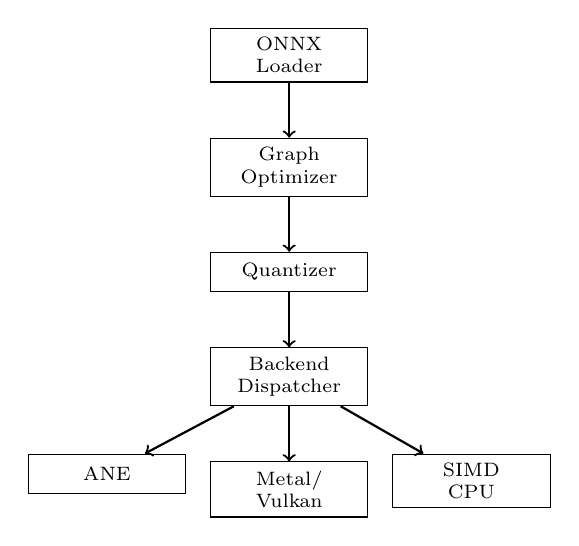
\begin{tikzpicture}[
    node distance=0.7cm,
    box/.style={rectangle, draw, minimum width=2cm, minimum height=0.5cm, align=center, font=\scriptsize},
    arrow/.style={->, thick}
]
\node[box] (onnx) {ONNX\\Loader};
\node[box, below=of onnx] (optimize) {Graph\\Optimizer};
\node[box, below=of optimize] (quant) {Quantizer};
\node[box, below=of quant] (dispatch) {Backend\\Dispatcher};
\node[box, below left=0.6cm and 0.3cm of dispatch] (ane) {ANE};
\node[box, below=of dispatch] (gpu) {Metal/\\Vulkan};
\node[box, below right=0.6cm and 0.3cm of dispatch] (cpu) {SIMD\\CPU};

\draw[arrow] (onnx) -- (optimize);
\draw[arrow] (optimize) -- (quant);
\draw[arrow] (quant) -- (dispatch);
\draw[arrow] (dispatch) -- (ane);
\draw[arrow] (dispatch) -- (gpu);
\draw[arrow] (dispatch) -- (cpu);
\end{tikzpicture}
\caption{Edge inference pipeline from ONNX to hardware execution.}
\label{fig:edge}
\end{figure}

The Edge runtime processes models through a four-stage pipeline (Figure~\ref{fig:edge}): ONNX graph loading, optimization passes, optional quantization, and hardware dispatch. Each stage produces an intermediate representation that the next stage consumes.

\subsection{Hardware Abstraction Layer}

The backend dispatcher selects the execution backend based on hardware capabilities and model requirements:

\begin{lstlisting}[language=Rust]
pub trait Backend: Send + Sync {
    fn name(&self) -> &str;
    fn supports(&self, op: &OpType) -> bool;
    fn execute(
        &self,
        graph: &OptimizedGraph,
        inputs: &[Tensor],
    ) -> Result<Vec<Tensor>>;
    fn max_memory(&self) -> usize;
}
\end{lstlisting}

For heterogeneous execution, the dispatcher can split a graph across backends: attention layers on ANE, embedding lookups on CPU, and output projection on GPU. Graph partitioning uses a cost model calibrated per device family.

\subsection{Model Format}

Edge uses a custom binary format (\texttt{.hze}) that memory-maps weight tensors directly into the inference address space:

\begin{lstlisting}[language=Rust]
pub struct EdgeModel {
    header: ModelHeader,    // 64 bytes
    graph: ComputeGraph,    // operator DAG
    weights: MmapSlice,     // mmap'd tensors
    quantization: QuantInfo, // scale/zero-point
}
\end{lstlisting}

Memory mapping avoids copying weights into heap memory, reducing peak memory usage and enabling instant model loading.

\section{Key Features}

\subsection{Dynamic Quantization}

Edge supports post-training quantization without a calibration dataset:

\paragraph{INT8.} Per-channel symmetric quantization for weights, per-tensor asymmetric for activations:
\begin{equation}
    x_q = \text{clamp}\left(\text{round}\left(\frac{x}{s}\right) + z, 0, 255\right)
\end{equation}
where $s$ is the scale factor and $z$ is the zero point, computed from running min/max statistics.

\paragraph{INT4.} Group-wise quantization with groups of 32 elements, achieving 8x compression with acceptable quality loss for language models.

\subsection{Operator Fusion}

The optimizer implements 12 fusion patterns:

\begin{itemize}
    \item Conv + BatchNorm + ReLU $\rightarrow$ FusedConvBNReLU
    \item MatMul + Add + GELU $\rightarrow$ FusedLinearGELU
    \item Multi-Head Attention (Q/K/V projections + softmax + output) $\rightarrow$ FusedAttention
    \item LayerNorm + Linear $\rightarrow$ FusedNormLinear
\end{itemize}

Fused operators reduce memory bandwidth requirements by avoiding materialization of intermediate tensors.

\subsection{Apple Neural Engine Support}

On Apple Silicon, Edge compiles eligible subgraphs to ANE via the Core ML backend. ANE is preferred for:

\begin{itemize}
    \item Convolutions (2x--5x faster than GPU for common sizes)
    \item Matrix multiplications with batch size 1 (inference)
    \item Transformer attention blocks
\end{itemize}

Operations unsupported by ANE (custom activations, dynamic shapes) fall back to Metal GPU or NEON CPU.

\section{Implementation}

Edge is implemented in 22,000 lines of Rust with platform-specific backends: 3,000 lines of Metal shader code (Apple), 2,500 lines of Vulkan compute shaders (Android/Linux), and 1,500 lines of NEON/AVX intrinsics (CPU).

\section{Status of the performance figures}
\label{sec:figures}

An earlier version of this paper carried a table titled ``Inference latency on
iPhone 15 Pro'' reporting 8\,ms for MobileNet-V3, 1.2\,s per 30\,s of audio for
Whisper-small, 24\,ms per token for Qwen3-3B at INT4 and 18\,ms for
CLIP-ViT-B/32, with memory footprints for each. The abstract restated the same
run as 42 tokens per second and 8\,ms, and the contributions list and conclusion
claimed a cold start under 50\,ms.

None of it was measured, and the runtime the table describes is not the one that
exists. \texttt{hanzoai/edge} is a Candle-based Rust crate with no iOS target,
no Core~ML or Neural Engine backend, no ONNX loader, and none of the four models
named in the table; its own \texttt{bench} subcommand reports time-to-first-token
and tokens per second for an already-loaded model and never measures load time.
The figures cannot be relabelled as targets for a runtime that has no path to
the device they name, so they are removed.

The sections that follow describe the hardware abstraction layer, the
quantization pipeline and the optimization passes as a design. Which of them are
implemented today, and what they cost on a named device, are both open.

\section{Security}

\paragraph{Model Protection.} Model weights can be encrypted with a device-specific key derived from the Secure Enclave (iOS) or Keystore (Android). The key never leaves the secure hardware.

\paragraph{Input Privacy.} All inference runs on-device. No input data, intermediate activations, or results are transmitted to external servers.

\paragraph{Memory Safety.} Rust's ownership model prevents buffer overflows, use-after-free, and data races. The \texttt{unsafe} blocks are limited to hardware-specific FFI calls and SIMD intrinsics, totaling less than 5\% of the codebase.

\paragraph{Sandboxed Execution.} On iOS, Edge runs within the app sandbox. On Android, it uses SELinux confinement. On Linux/IoT, seccomp filters restrict system calls to file I/O and memory allocation.

\section{Conclusion}

Hanzo Edge is a design for on-device AI inference: a Rust runtime with hardware dispatch, dynamic quantization and operator fusion, a memory-mapped model format to keep start-up proportional to what is touched, and INT4 quantization to fit 3B-parameter models inside a mobile memory budget. Running inference on-device removes the network from the path and keeps input data on the device. What the design costs in latency and memory on a named device is not established here; Section~\ref{sec:figures} says why the previous figures were withdrawn.

\bibliographystyle{plain}
\begin{thebibliography}{10}

\bibitem{onnx2017}
ONNX. Open Neural Network Exchange. 2017.

\bibitem{jacob2018}
B. Jacob et al. Quantization and Training of Neural Networks for Efficient Integer-Arithmetic-Only Inference. CVPR, 2018.

\bibitem{coreml2017}
Apple. Core ML: Integrate machine learning models into your app. 2017.

\bibitem{gholami2022}
A. Gholami et al. A Survey of Quantization Methods for Efficient Neural Network Inference. arXiv:2103.13630, 2022.

\end{thebibliography}

\end{document}
